\documentclass[a4paper]{article}
\usepackage{forest}
\usepackage{float}
\usepackage{geometry}
\usepackage{makecell}
\usepackage{mathtools, nccmath}
\usepackage{amsmath}
\usepackage{listings}
\usepackage{hyperref}
\usepackage{graphicx}
\usepackage{ragged2e}
\usepackage{color}
\usepackage{xepersian}
\usepackage{subfiles}
\DeclareMathSizes{12}{30}{16}{12}
\newgeometry{left=1.4cm, right=1.4cm, bottom=2.0cm, top=2.0cm}
\settextfont[Scale=1]{XB Roya}

\DeclareMathSizes{12}{30}{16}{12}
\newgeometry{left=1.4cm, right=1.4cm, bottom=2.0cm, top=2.0cm}
\settextfont[Scale=1]{XB Roya}
\renewcommand{\baselinestretch}{1.5}

\newcommand{\equate}[1]{
    \begin{fleqn}
        \begin{gather}
            #1
        \end{gather}
    \end{fleqn}
}

\title{گزارش ارزیابی کارایی سیستم‌های اینترنت اشیا پزشکی و اینترنت اشیا براساس
مجموعه داده‌های \lr{CICIoMT2024} و مدلینگ ریاضیاتی \\ استاد ناظر: آقای دکتر مهدی
امینیان}
\author{علیرضا سلطانی نشان}

\begin{document}
\maketitle

\section*{مجوز}

به فایل license همراه این برگه توجه کنید. این برگه تحت مجوز GPLv3 منتشر شده است
که اجازه نشر و استفاده (کد و خروجی/pdf) را رایگان می‌دهد.

\tableofcontents
\listoffigures
\listoftables

مهم‌ترین انگیزه برای توسعه این تحقیق وجود کمبود در داده‌های موجود ارزیابی کارایی
تجهیزات اینترنت اشیا پزشکی و پیشرفت امنیتی تمام شبکه‌هایی که در خصوص جریان‌های
داده‌ای و پردازش داده‌های پزشکی کار می‌کنند، می‌باشد بخصوص برای دستگاه‌های
اینترنت اشیا پزشکی به دلیل اطلاعات حیاتی‌ای که می‌توان به واسطه آن‌ها از بیماران
با بیماری‌های مختلف مانیتور و دریافت کرد.

% TODO: Write about CICIoMT2024
\newpage

\section{رابطه مدل‌های ریاضی با شاخص‌های کلیدی کارایی}

برای مدل‌سازی جهت ارزیابی عملکرد سیستم‌های مختلف از قبیل سیستم‌های \lr{IoT}
بایستی شاخص‌های کلیدی کارایی یا \lr{KPI} \footnote{\lr{Key Performance
Indicators}} را بشناسیم. این \lr{KPI}ها شامل مجموعه‌ای از فرمول‌های ریاضیاتی
هستند که نسبت به نیازمندی‌های غیرعملیاتی یا \lr{Non-functional requirements}
متفاوت می‌باشند. نیازمندی‌های غیرعملیاتی مانند میزان مصرف انرژی، میزان مصرف
حافظه، سرعت انتقال اطلاعات و گذردهی، میزان دقت، میزان دردسترس بودن، میزان قابلیت
اطمینان و غیره می‌باشد. برای هر کدام از این نیازمندی‌های غیرعملیاتی فرمول‌هایی
وجود دارد که می‌تواند با فراگیری آن‌ها به مقادیری رسید که در مرحله بعد می‌توان
آن‌ها را در مدل‌های ریاضیاتی استفاده کرد.  مرحله دوم در حقیقت ارزیابی کارایی
سیستم‌ها با استفاده از مدل‌های شناخته شده ریاضیاتی می‌باشد که رابطه مستقیمی با
\lr{KPI}‌ها دارند. یعنی ‌نمی‌توان مقادیر \lr{KPI} را برای این مدل‌ها نادیده
گرفت. در نهایت با مدل‌های مطرح شده می‌توان کارایی سیستم‌های \lr{IoT} در
دامنه‌های مختلف را ارزیابی کرد و بین آن‌ها مقایسه و \lr{Trade off} نسبت به
\lr{Benchmark}های بدست آمده انجام داد.

\lr{KPI}ها و مدل‌هایی که در این گزارش مورد بررسی قرار گرفته‌اند:

\subsection{\lr{KPI}ها}

% TODO: Write after review
\begin{itemize}
    \item 
\end{itemize}

\subsection{مدل‌ها}

\begin{itemize}
    \item 
\end{itemize}

یکپارچه‌سازی سیستم‌های IoT با سیستم‌های ابری چالش‌های زیادی داشته مثل:

\begin{itemize}
    \item تاخیر‌های شبکه‌ای
    \item گذردهی
    \item مصرف انرژی
    \item قابلیت اطمینان
\end{itemize}

یه سری مفاهیم جدیدی در حوزه پردازش‌ها مطرح شده که حتی می‌تواند کاربرد‌های مختلفی
در استفاده از اینترنت اشیا باشه. این مفاهیم جدید مثل \lr{Fog computing},
\lr{edge computing}, \lr{mobile edge computing}, \lr{mobile cloud computing} و
\lr{Cloudlet} ‌ها هستش.  در این مقاله یک مدل ریاضیاتی برای توصیف رسمی سیستم‌های
\lr{IoT} ارائه داده شده است.  علاوه‌بر این یک ارزیابی آنالیز شده برای طراحی این
سیستم‌ها با استفاده از مطابقت با معماری، تکنولوژی‌ها، پروتکل‌ها و مدل‌های
یکپارچه‌سازی برای بهینه‌سازی عملکرد نیز ارائه می‌دهد.

\lr{Approach of this article:}

بعد از خوندن این مقاله به یک روش بهینه برای بهینه‌سازی کارایی مبتنی بر
فرایند‌های \lr{offloading} مانند \lr{load balancing} آشنا می‌شیم.

مدلینگ ریاضیاتی سیستم‌های IoT یک نمایی از سیستم ایجاد می‌کنند که به فهمیدن
المان‌ها، تعاملاتشون، و رفتار‌هاشون کمک می‌کند.

\begin{enumerate}
    \item مدل مفهومی یا \lr{conceptual model} یک ساختار سطح بالایی برای توصیف
    عملیاتی است که در سیستم‌های IoT انجام می‌شود.
    \item مدل رفتاری یا \lr{behavioral model} ممکنه شامل جزیئیات باشه. مثل جریان
    داده بین المان‌ها.
\end{enumerate}

به طور کلی مودلینگ به مشخص شدن و پاسخ به مسائل مربوط به کارایی کمک بسزایی می‌کنه
و اجازه میده که سیستم‌ها بهینه‌تر، کاراتر و مطمئن‌تر باشن.

هر موقع در مورد مودلینگ یک سیستم IoT صحبت میشه در حقیقت قراره یه چهارچوبی درست
بشه که بتونیم باهاش تست کنیم، تایید یا validation انجام بدیم و یا بتوانیم سیستم
را به تقاضا‌هایی که داریم optimize کنیم.

فرایند سیستم‌های IoT معمولاً شامل شناسایی، دریافت اطلاعات (Sensing)، فعالیت‌های
تحت شبکه، و محاسبات کوچک هستش که باعث میشه با محیط فیزیکی و هر اشیایی ارتباط
برقرار کند.

در این مقاله سیستم‌های IoT با کاربردی که دارند به ۴ دسته تقسیم می‌شوند:

\begin{figure}[H]
  \centering
  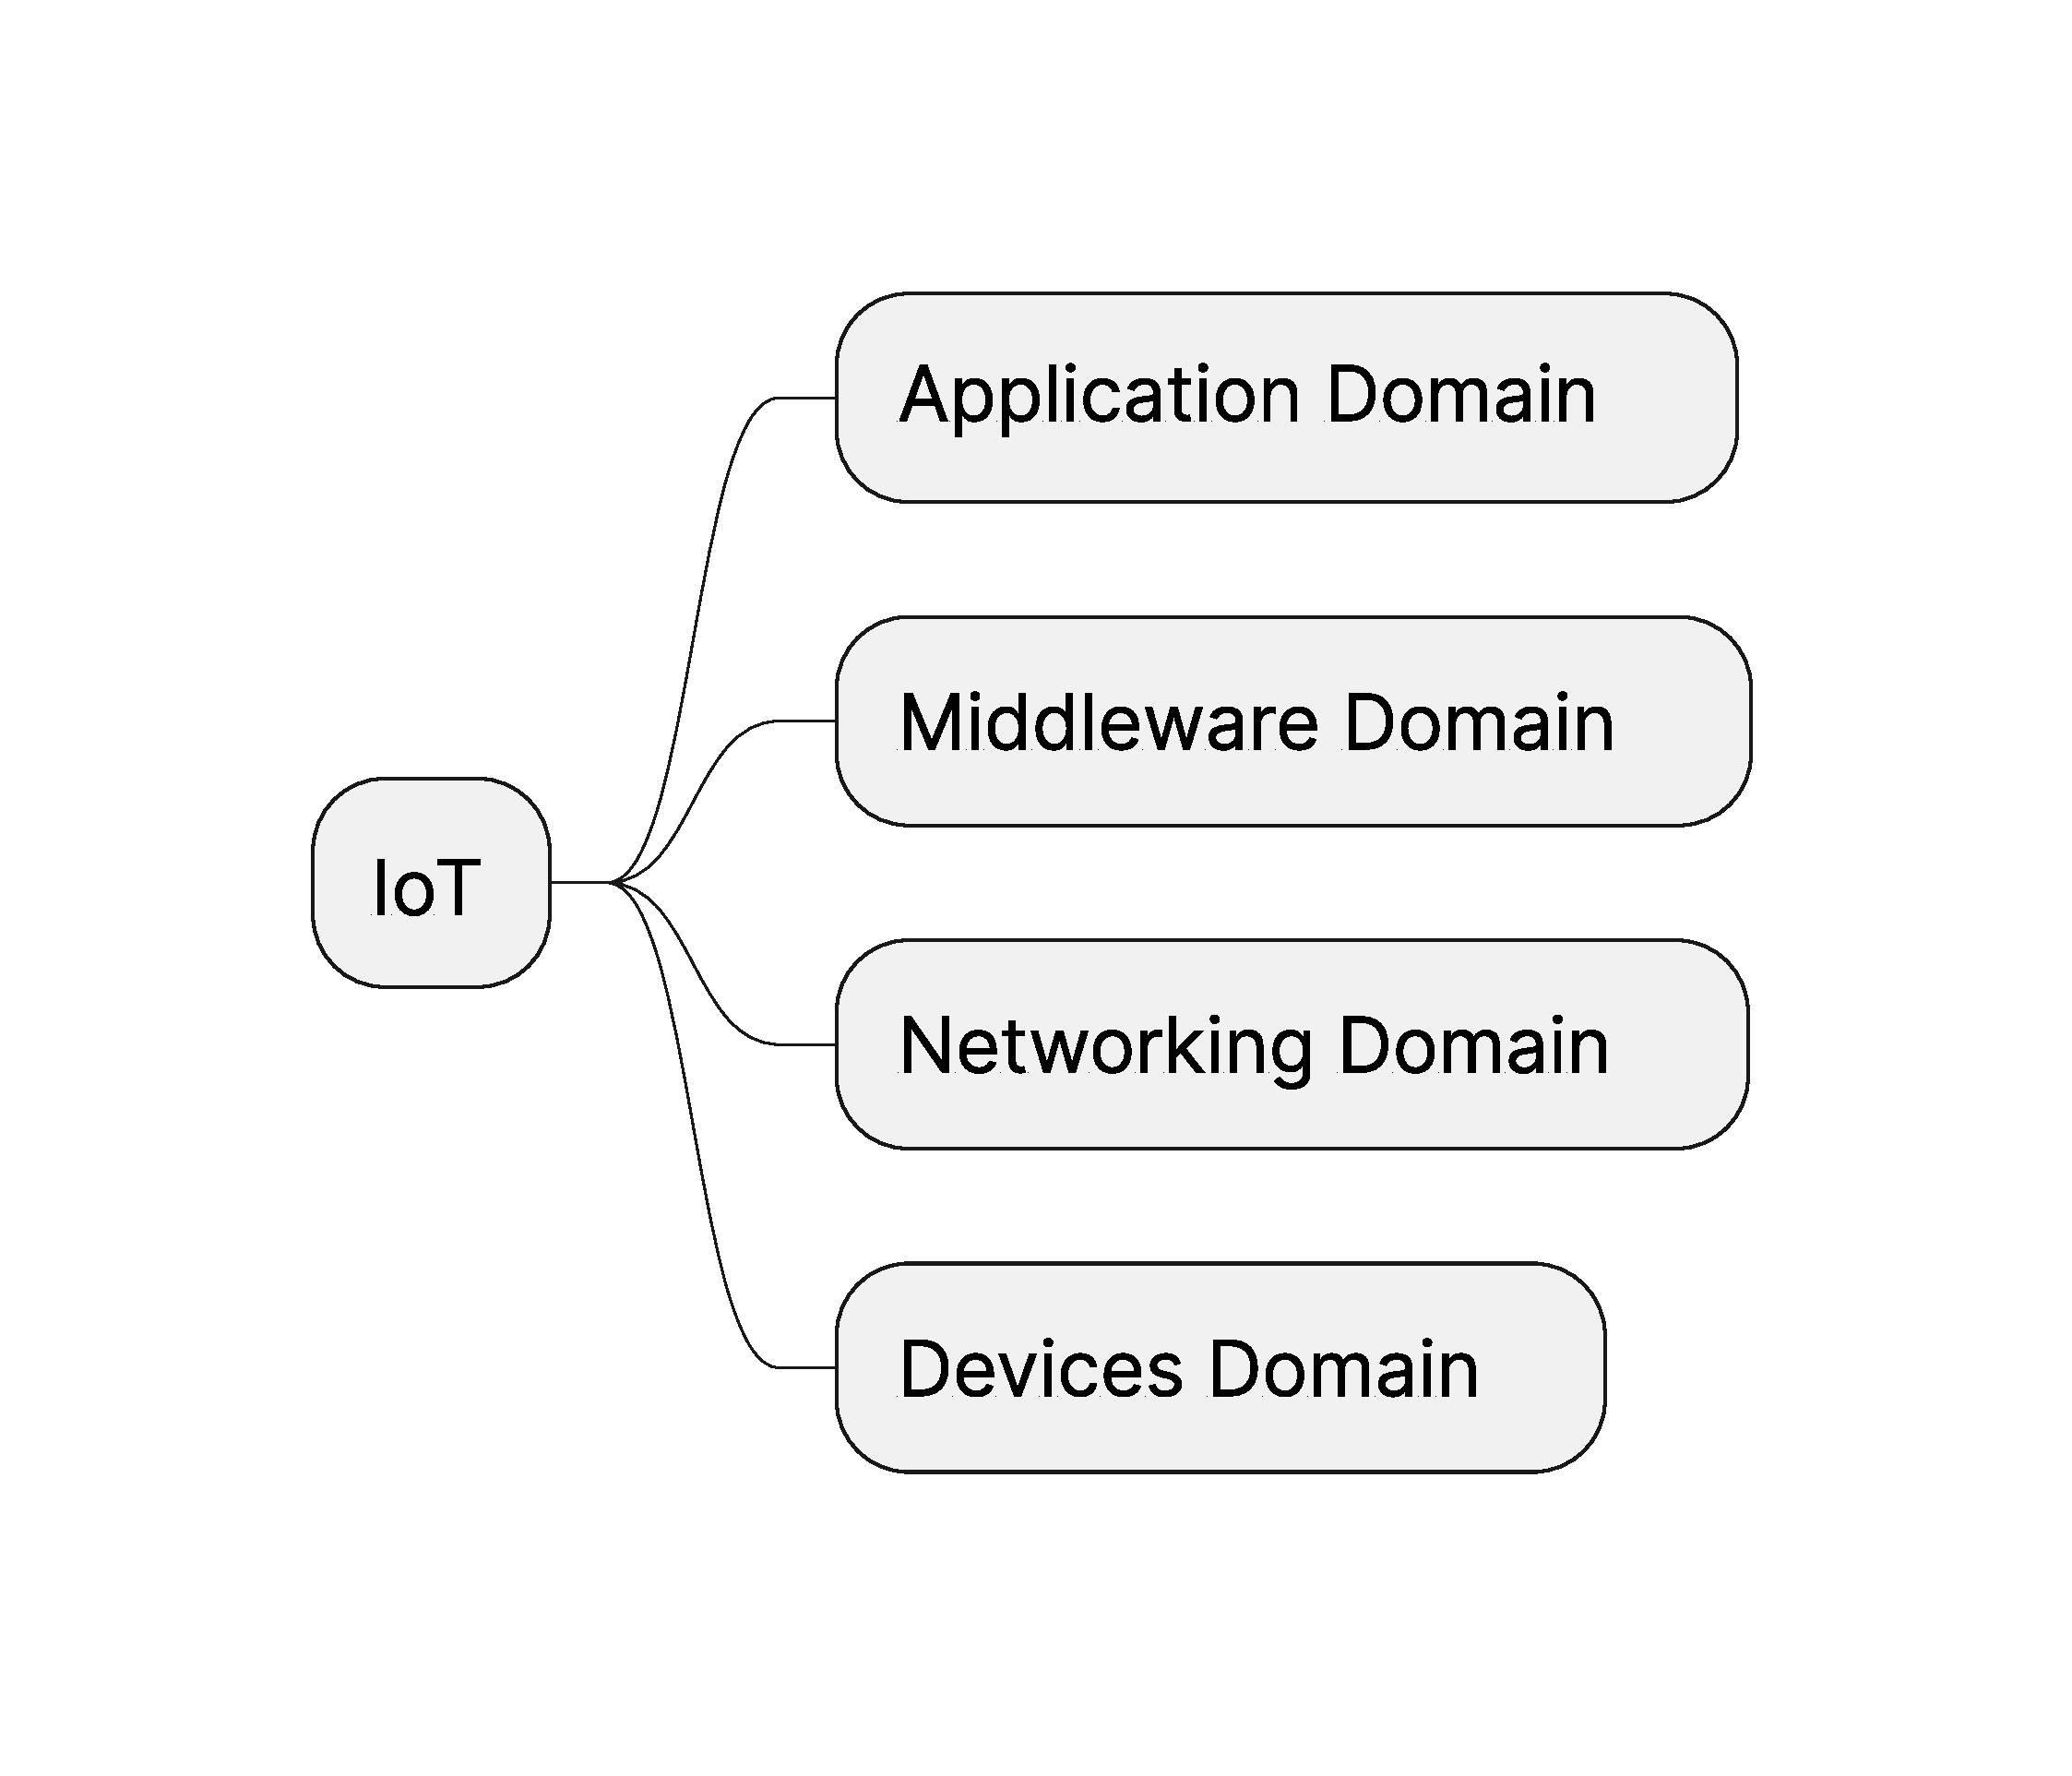
\includegraphics[width=0.6\textwidth]{./figures/IoT_overall_domains.pdf}
  \caption{۴ دسته‌بندی دامنه استفاده از سیستم‌های \lr{IoT}}
  \label{fig:iotOverallDomains}
\end{figure}

\begin{figure}[H]
  \centering
  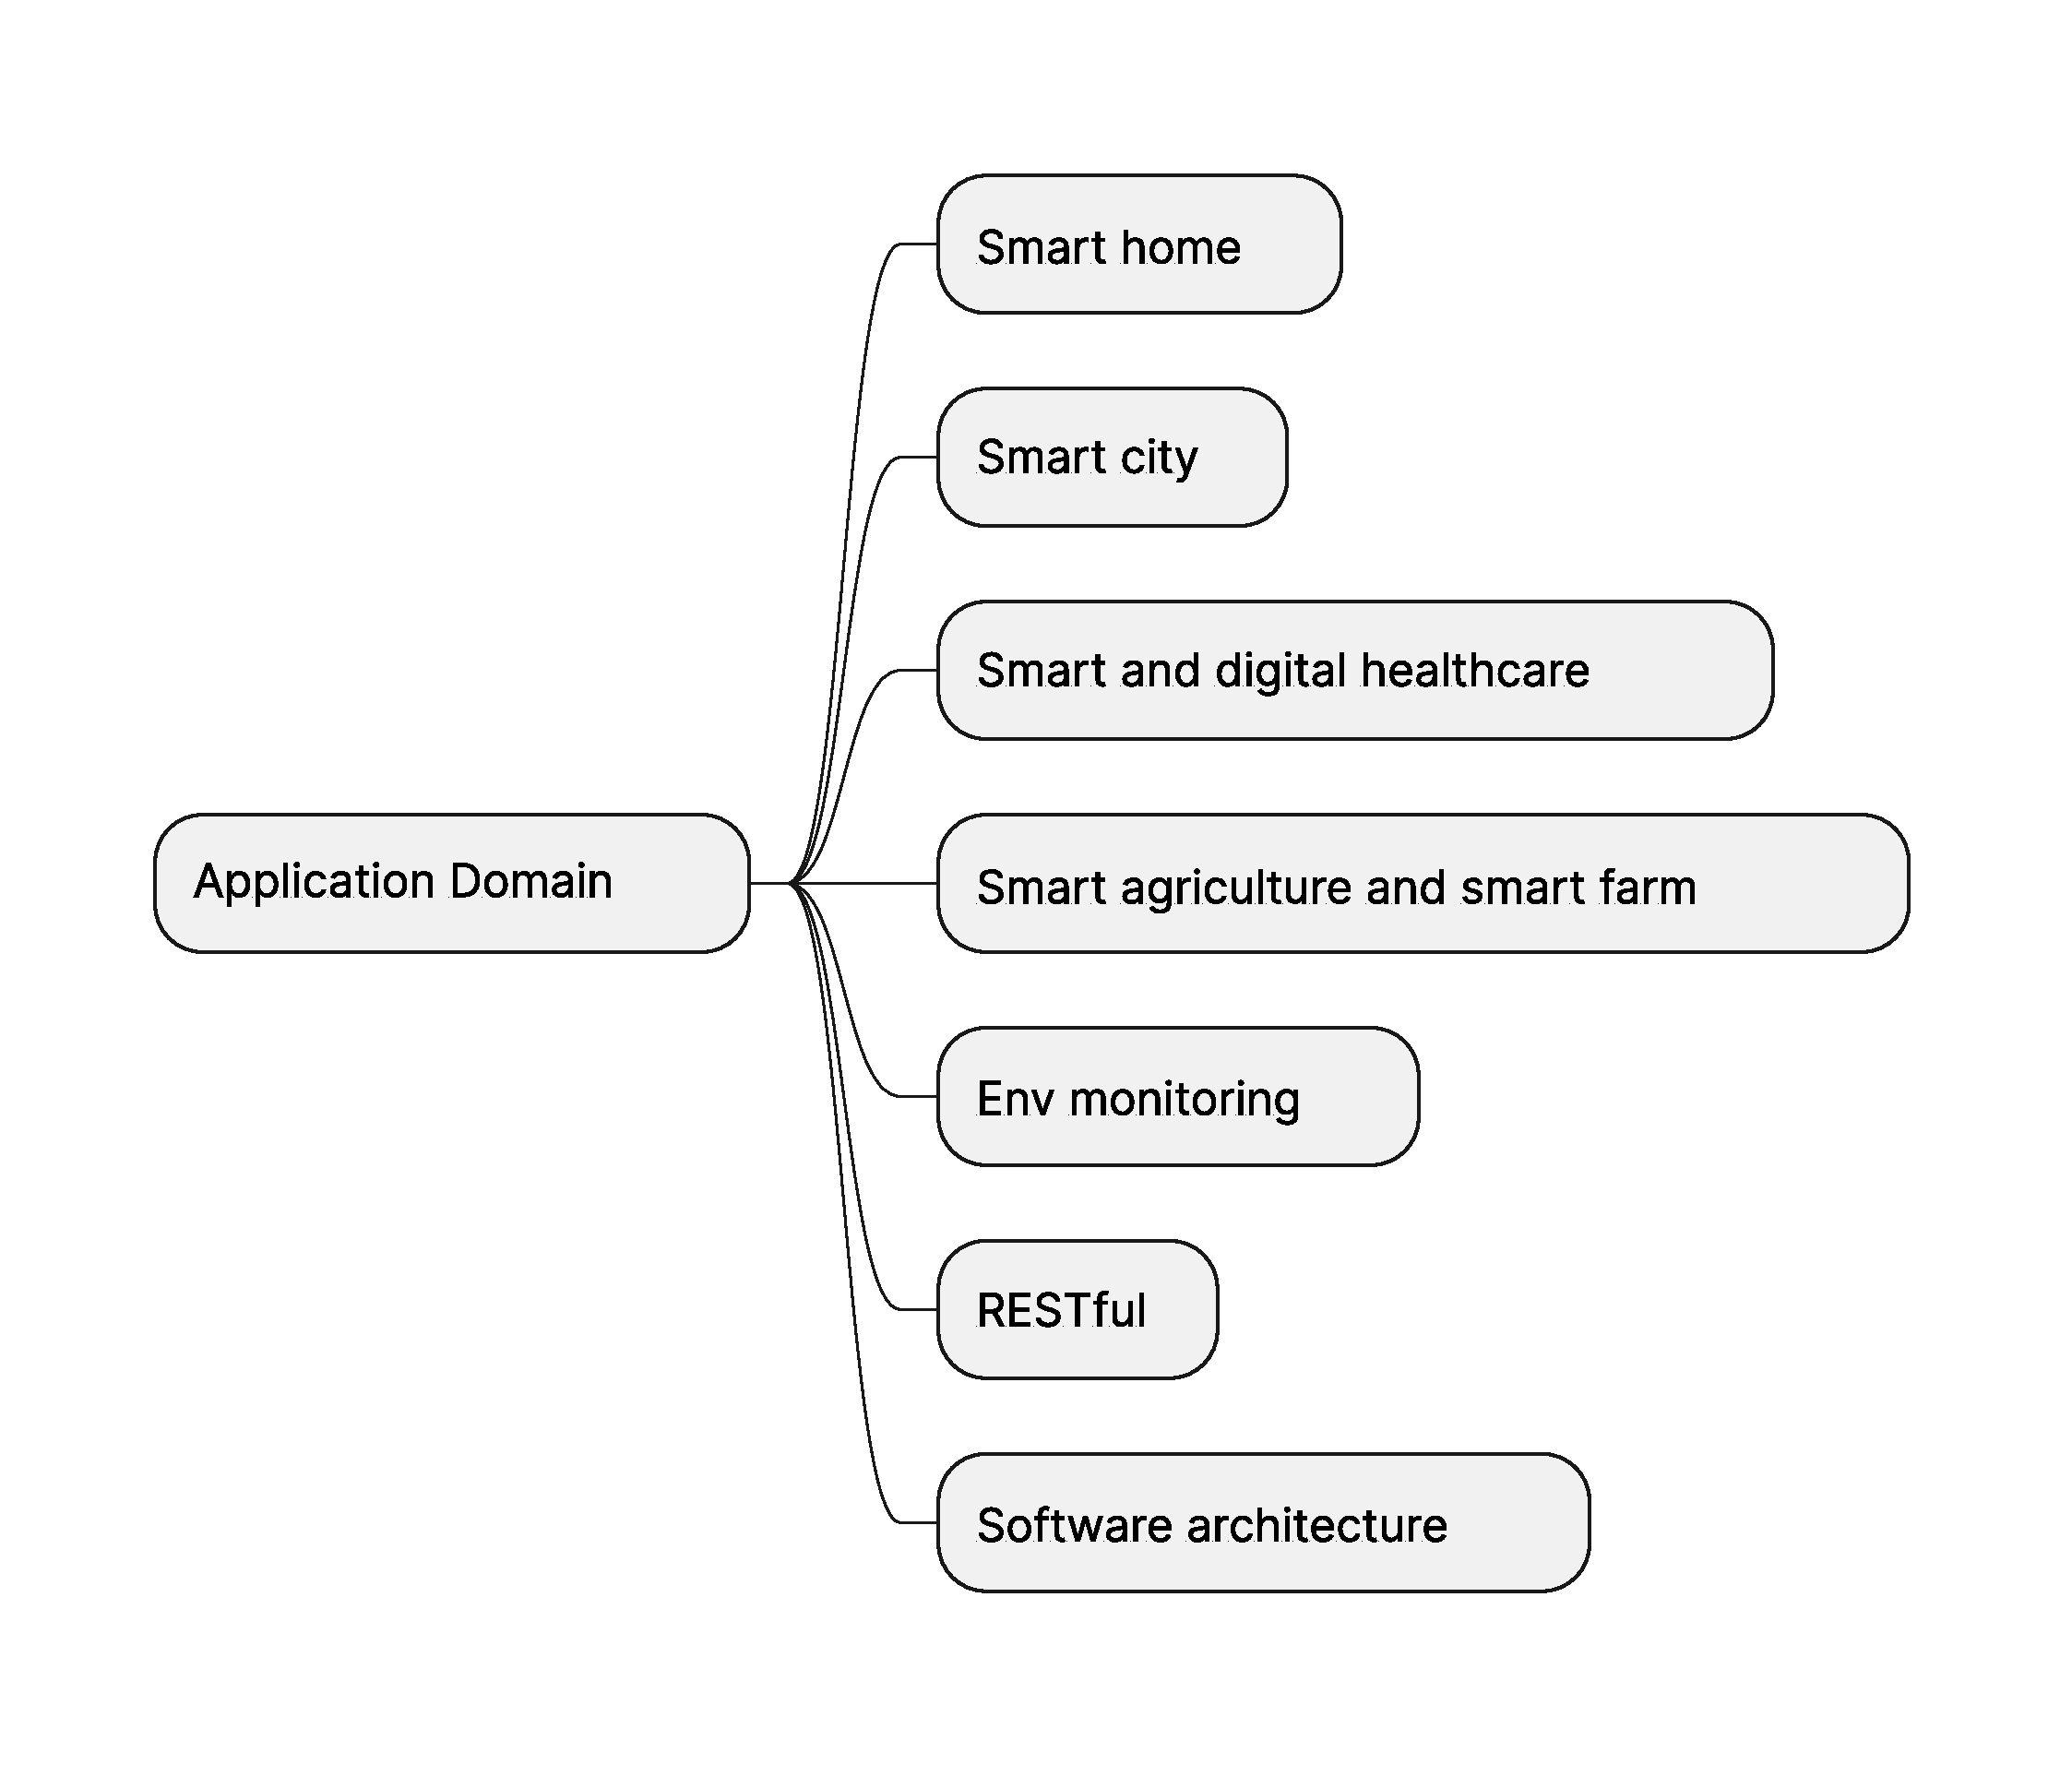
\includegraphics[width=0.9\textwidth]{./figures/IoT_application_domains.pdf}
  \caption{حوزه‌های تخصصی بخش اپلیکیشن در \lr{IoT}}
  \label{fig:iotApplicationDomains}
\end{figure}

\begin{figure}[H]
  \centering
  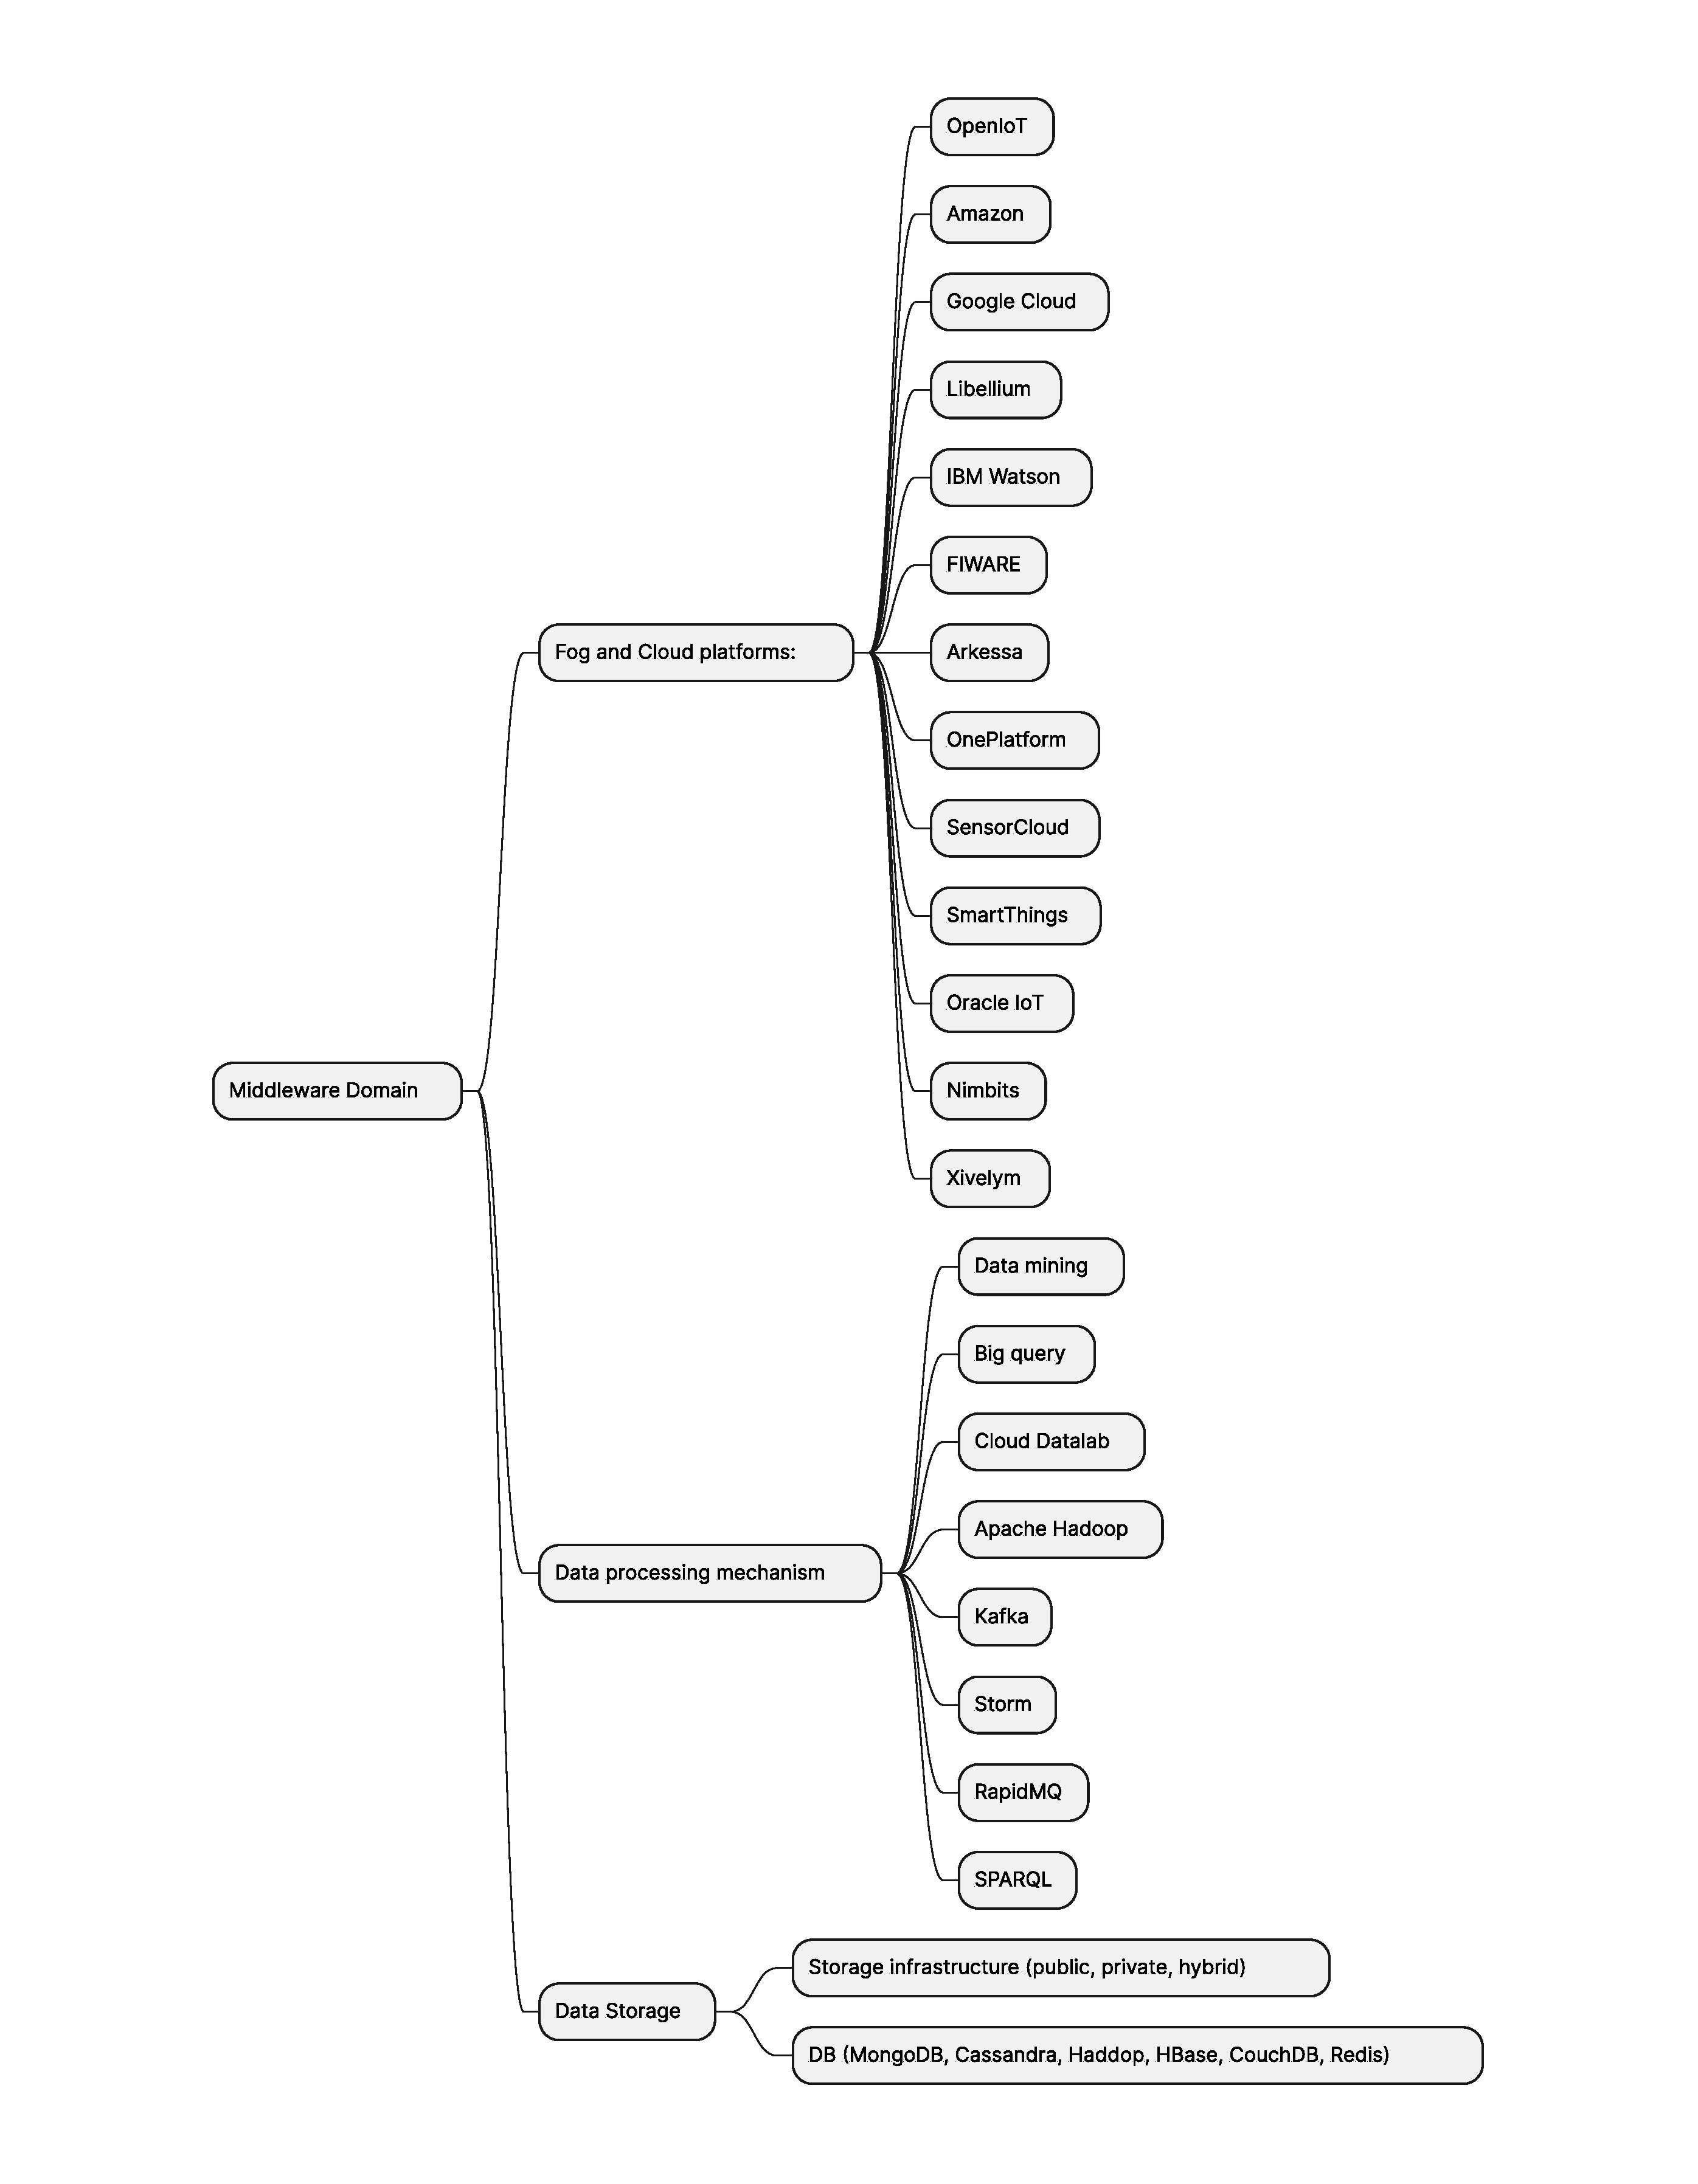
\includegraphics[width=0.9\textwidth]{./figures/IoT_middleware_domains.pdf}
  \caption{حوزه‌های بخش میان‌افزار در \lr{IoT}}
  \label{fig:iotMiddlewareDomains}
\end{figure}

\begin{figure}[H]
  \centering
  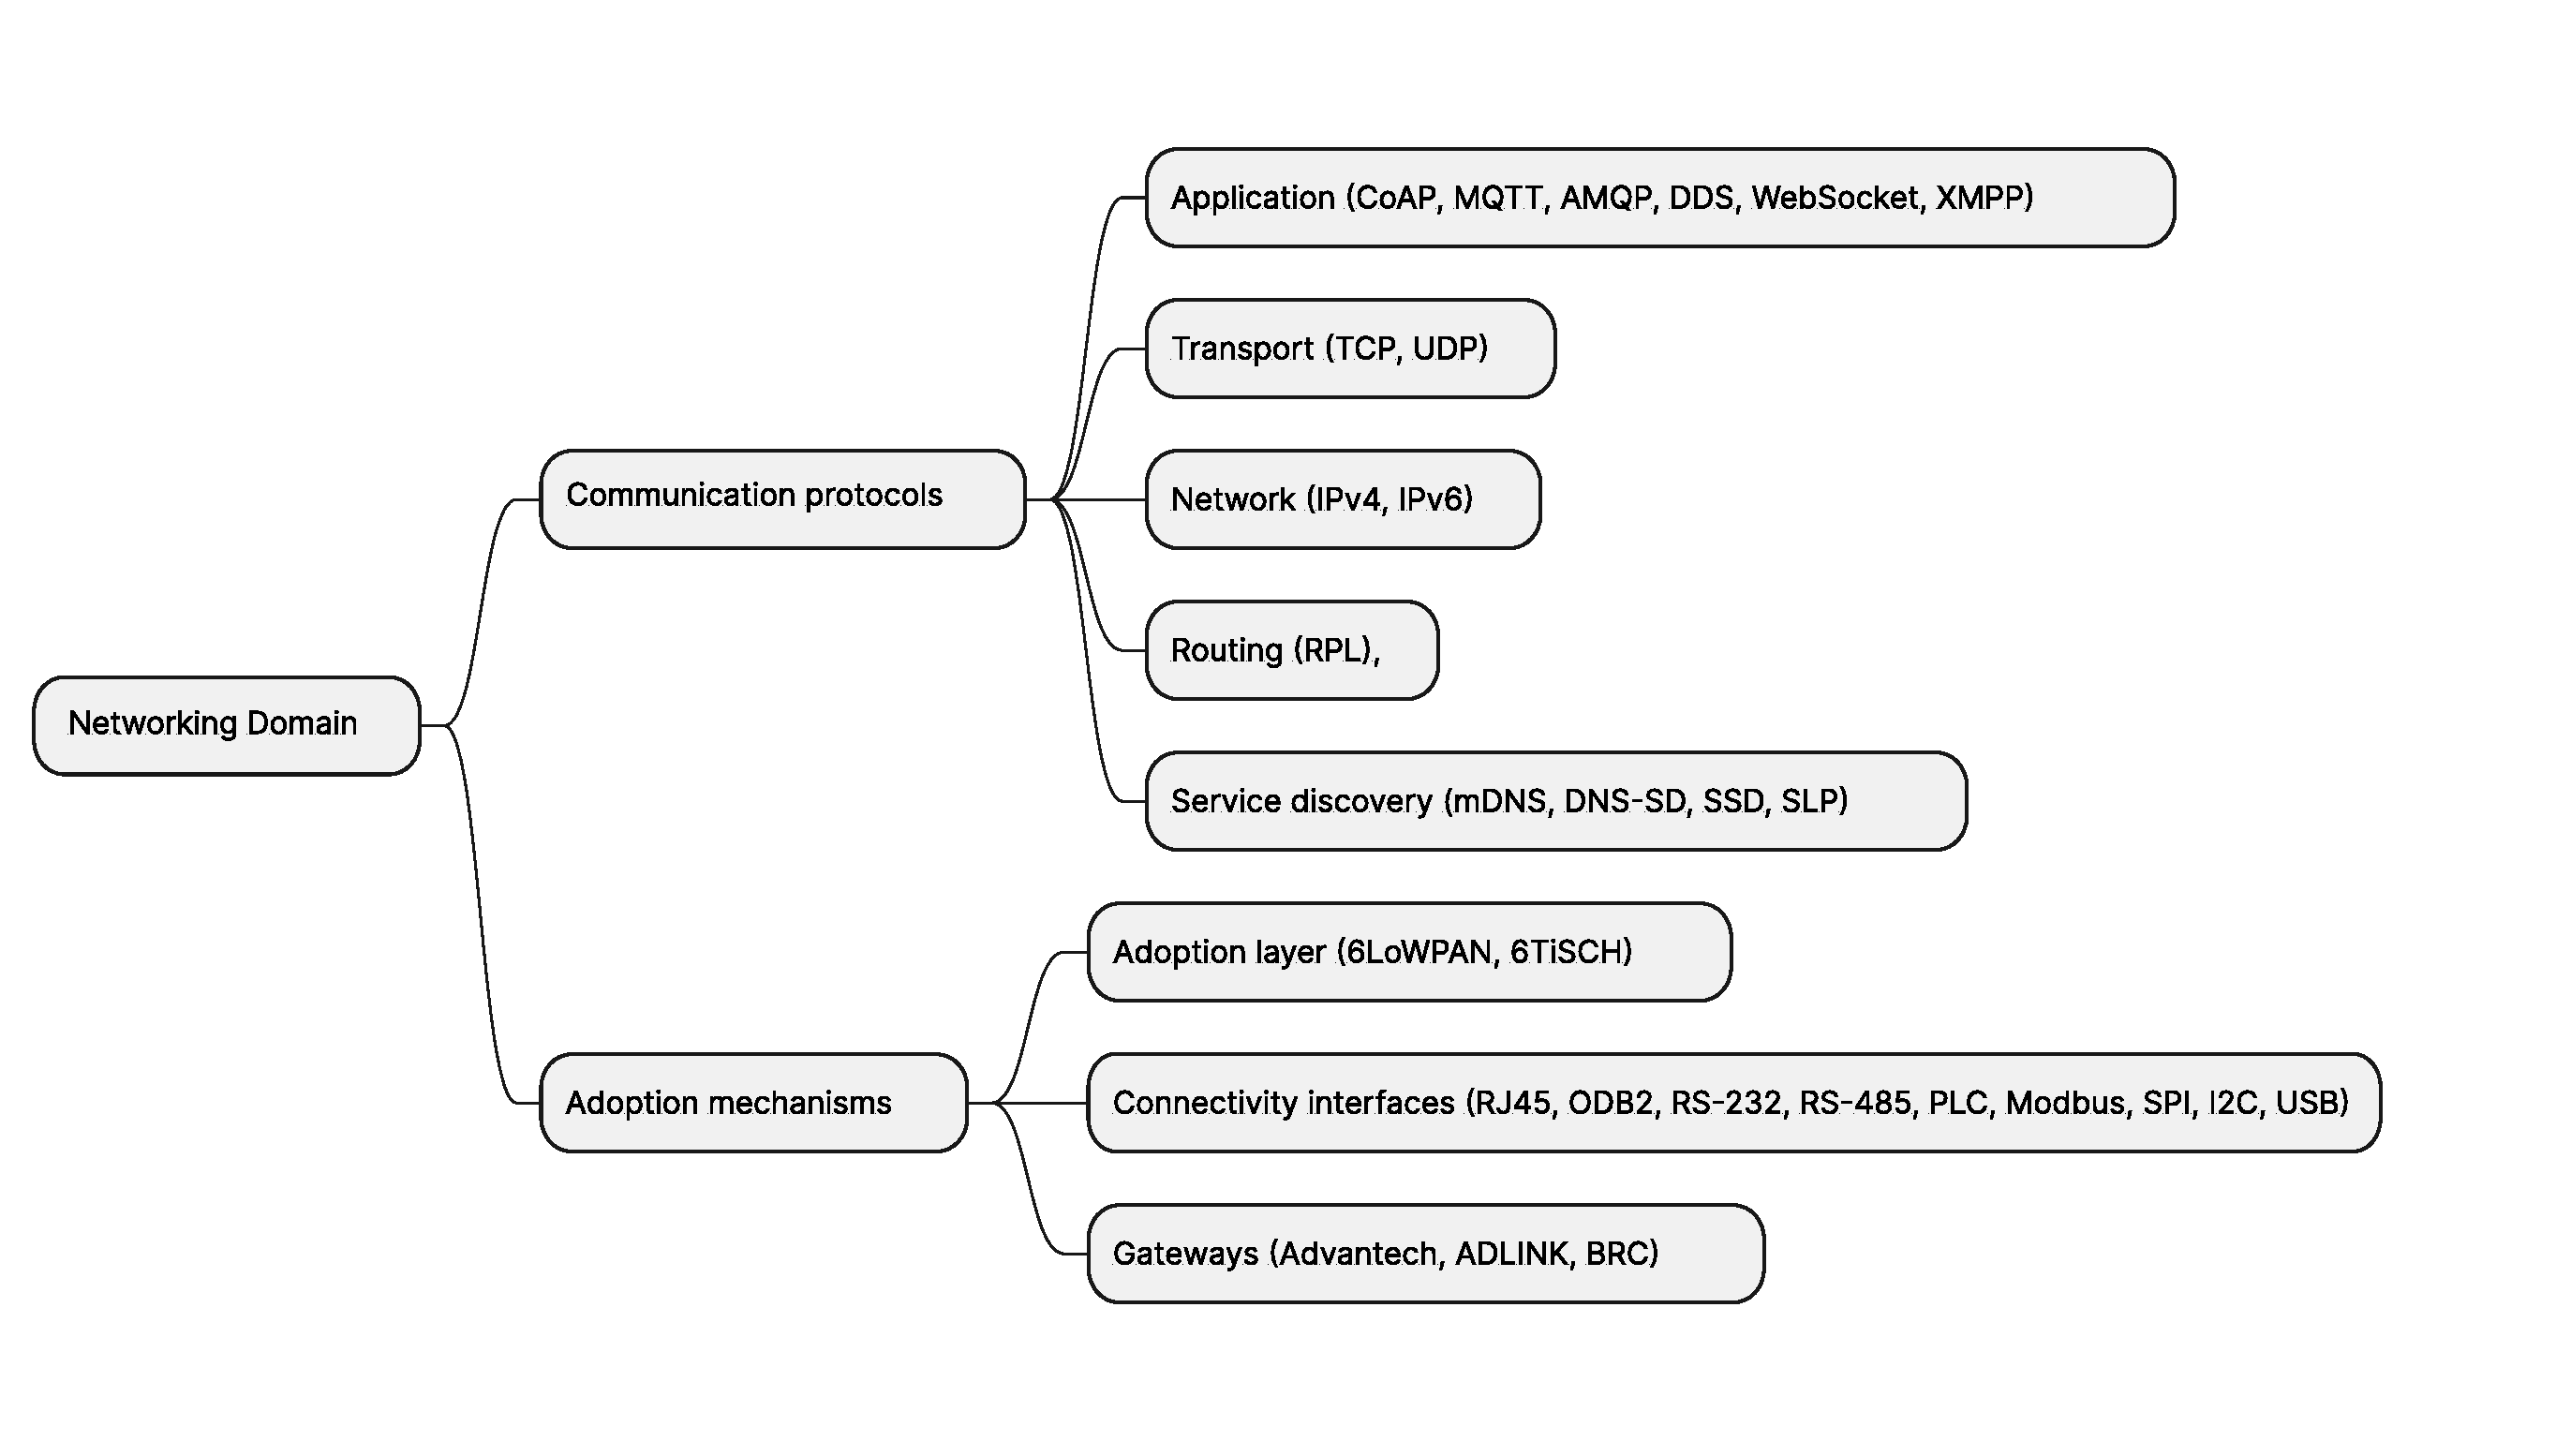
\includegraphics[width=0.9\textwidth]{./figures/IoT_network_domains.pdf}
  \caption{حوزه‌های بخش شبکه در \lr{IoT}}
  \label{fig:iotNetworkingDomains}
\end{figure}

\begin{figure}[H]
  \centering
  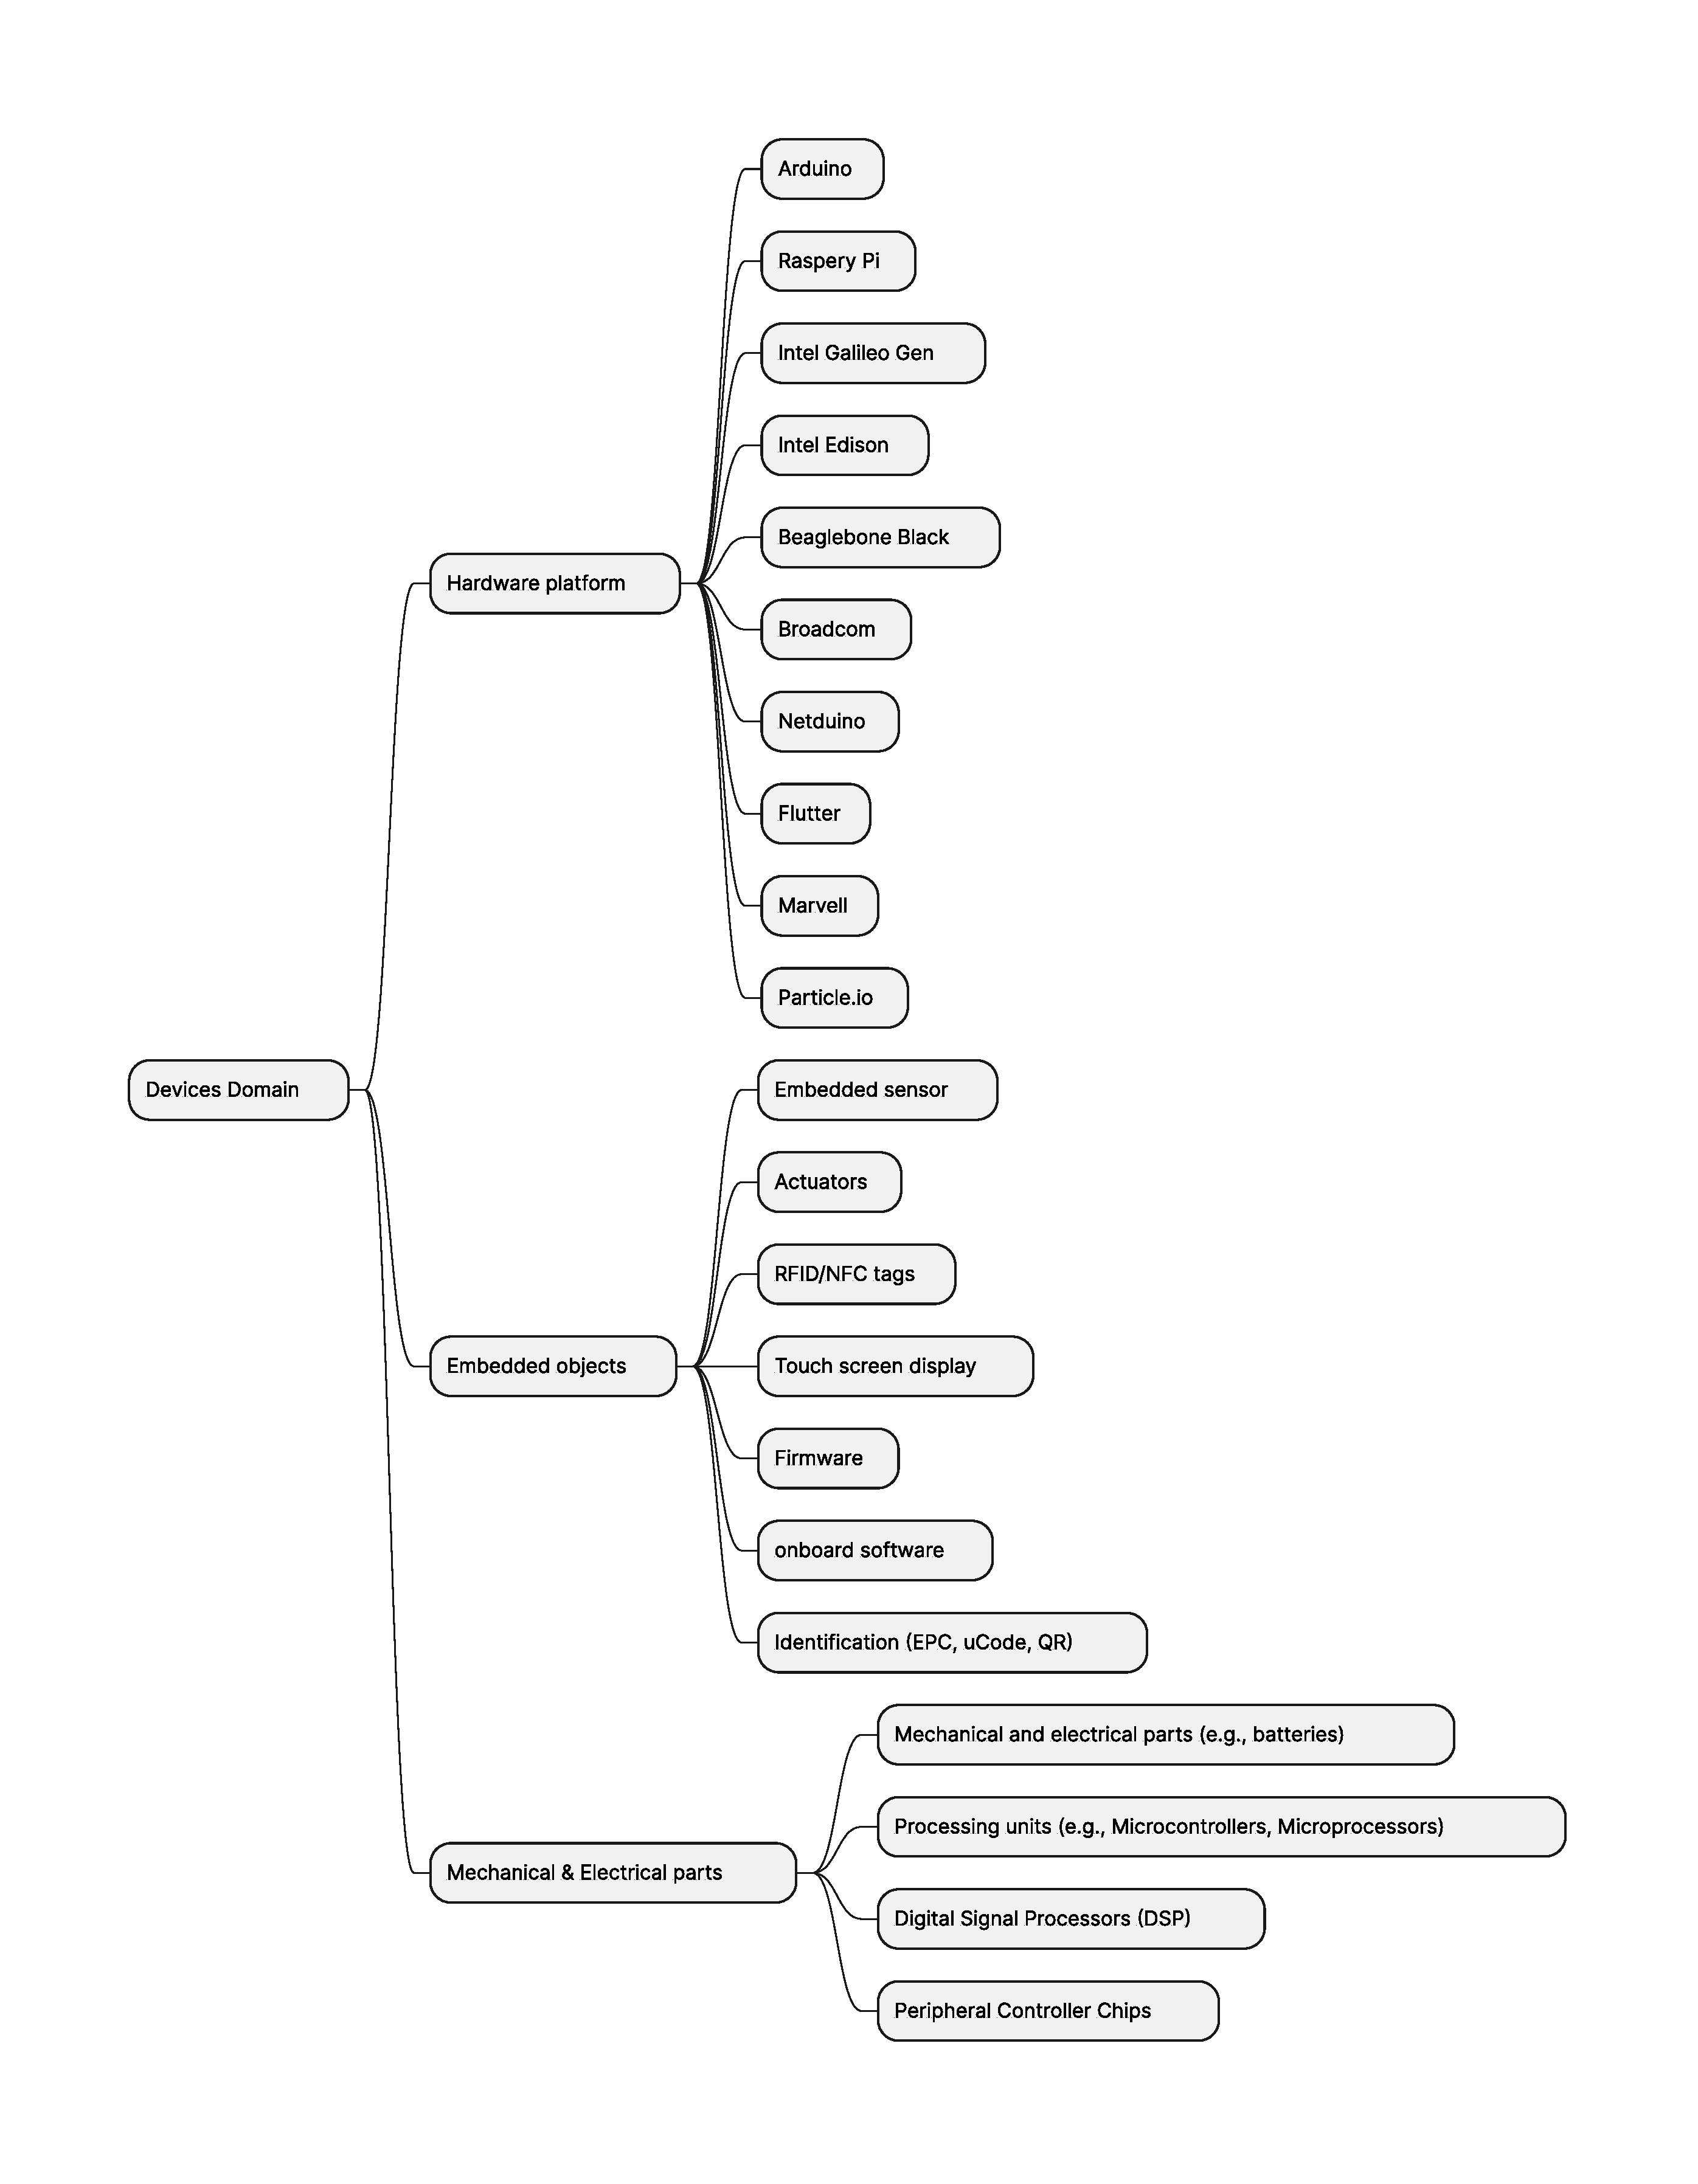
\includegraphics[width=0.9\textwidth]{./figures/IoT_devices_domains.pdf}
  \caption{حوزه‌های بخش \lr{Embedded} در \lr{IoT}}
  \label{fig:iotDevicesDomains}
\end{figure}

عمومیت جریان داده در سیستم‌های IoT:

\begin{itemize}
    \item دریافت داده
    \item انتقال داده
    \item پردازش داده
    \item ذخیره‌سازی داده
    \item آنالیز و معنادار کردن داده
\end{itemize}

\section{شاخش‌های محاسبه و ارزیابی عملکرد}

\begin{table}[H]
    \centering
    \scalebox{0.9}{
      \begin{tabular}{|>{\raggedleft\arraybackslash}p{10cm} | >{\raggedright\arraybackslash}p{5cm}|}
        \hline
        \textbf{تعاریف} & \textbf{ثابت‌ها} \\ \hline
        نرخ ورود اطلاعات & $D_{rate}$ \\ \hline
        مصرف انرژی & $E_{dev}$ \\ \hline
        تاخیر سرویس‌دهی & $T_{exe.}$ \\ \hline
        مشخصات سیستم \lr{IoT} & $IoT_{sys_{sp}}$ \\ \hline
        زمان ورکلود‌ها & $t_{ws}$ \\ \hline
        تعداد دستگاه‌ها & $k$ \\ \hline
        درصد داده‌ای که در سیستم $i$ پردازش می‌شود & $\beta$ \\ \hline
        مقدار گذردهی & $\tau$ \\ \hline
        نیازمندی مشخص کارایی $P_{i_{req}}$ جایی که $P_{i}$ $i^{th}$ مقدار از کارایی است & $IoT_{sys}(P) = \{P_{i_{req}}, P_{i}\}$ \\ \hline
        مدت زمان سرویس‌دهی & $P_{i} = \langle T_{exe.}, E_{dev} \rangle$ \\ \hline
        مصرف انرژی داخلی & $E_{loc}$ \\ \hline
        انرزی مورد نیاز برای \lr{offloading} & $E_{off}$ \\ \hline
        انرژی مصرفی در زمان بیکاری & $E_{idle}$ \\ \hline
        پردازش تسک‌های داخل دستگاه & $P_L$ \\ \hline
        زمان پردازش تسک‌های داخلی & $t_L$ \\ \hline
      \end{tabular}
    }
    \caption{تعریف ثابت‌های مورد استفاده در فرمول‌ها}
    \label{table:staticAndDynamicComparison}
\end{table}

\subsection{فرمول شانون}

نرخ داده‌ها می‌تواند از طریق فرمول شانون محاسبه شود.

\equate{
    D_{rate} = B_{i,j} \log_{2} (1 + \frac{\lvert h_{ij} \rvert ^{2} . P_{tx}}{P_{Nj}}) 
}

\begin{itemize}
    \item $B_{ij}$: پهنای باند
    \item $h_{ij}$: بهره کانال بین دستگاه مبدا و مقصد که نشان می‌دهد سیگنال
    چگونه در مسیر بین فرستنده و گیرنده تقویت یا تضعیف می‌شود.
    \item $P_{tx}$: توان ارسال
    \item $P_{N}$: میزان نویز مقصد
\end{itemize}

کاربرد زیادی در سناریو‌هایی دارد که در آن یک ارسال کننده و یک دریافت کننده وجود
دارد.

\subsection{فرمول محاسبه بار سیستم یا \lr{System load}}

مجموع بار سیستم از طریق فرمول زیر بدست می‌آید:

\equate{
    D = \sum_{k = 1}^{N} D_{rate, k} \times T_{w, k}
}

\begin{itemize}
    \item $D_{rate, k}$: نرخ تولید داده توسط دستگاه \lr{IoT}
    \item $t_{w, k}$: مدت زمان ورودی در دستگاه \lr{IoT} یا به عبارتی دیگر، مدت
    زمانی که طول می‌کشد یک دستگاه \lr{IoT} ورودی را دریافت و سپس آن را پردازش و
    هندل کند.
\end{itemize}

\subsection{تاخیر سرویس‌دهی یا \lr{Service latency}}

مسئله \lr{service latency} یا \lr{service execution time ($T_{exe.}$)} مدت زمانی
است که طول می‌کشد سیستم \lr{IoT} تمام درخواست‌های پردازشی و ارتباطی را اجرا کند
\lr{(the total application exe time)}. مدت زمان کل مصرف شده از، مدت زمان سرویس
یک ریکوئست به مدت زمان تمام تسک‌هایی که با موفقیت پردازش شده‌اند. بنابراین، این
فاصله زمانی بین درخواست برنامه و بدست آوردن نتایج می‌باشد.

\subsubsection{بخش‌هایی که زمان سرویس‌دهی دارند}

\begin{itemize}
    \item مدت زمان انتقال داده از دستگاه IoT به زیر ساخت فاگ
    \item مدت زمان انتقال داده از دستگاه IoT به سرور‌های ابری
    \item مدت زمان انتقال داده از فاگ به کلاد
    \item مدت زمان انتقال اعلانات از کلاد به فاگ
    \item مدت زمان انتقال اعلانات از کلاد به دستگاه‌های IoT
    \item مدت زمان انتقال اعلانات از فاگ به دستگاه IoT
    \item مدت زمان محاسبات در دستگاه IoT
    \item مدت زمان محاسبات در لایه فاگ
    \item مدت زمان محاسبات در سرور‌های ابری
\end{itemize}

نکته: مدت زمانی که برای هر کاری در سیستم‌های \lr{IoT} سپری می‌شود به نوع و شیوه
پیاده‌سازی معماری دستگاه‌ها و نرم‌افزار بخش‌ها بستگی دارد و می‌تواند کاملاً
متفاوت باشند. عموماً سرویس لیتنسی بین المان‌های سیستم \lr{IoT} توزیع شده هستش و
شامل دستگاه‌های اینترنت اشیا، شبکه‌ها و سیستم‌های پردازشی می‌شود.

تاخیر سرویس‌دهی:

\equate{
    T_{exe.} = T_{cm} + T_{cp}
}

\begin{itemize}
    \item $T_{cm}$: مدت زمان تاخیر در ارتباطات
    \item $T_{cp}$:مدت زمان تخیر در پردازش
\end{itemize}

مدت زمان اجرا بایستی کمتر از زمان‌بندی تسک‌ها در فاگ یا کلاد باشد. یعنی سرویس
تایم باید کمتر از نیازمندی‌های \lr{IoT application ($T_req$)} باشد.

برای کاهش \lr{service latency} از فرمول زیر بایستی پیروی کند:

\equate{
    Objective: \min (T_{exe.}) = T_{cm} + T_{cp} \leq T_{req}
}

موقعی که داری در مورد \lr{Execution time} می‌نویسی فرمول \lr{communication
latency} رو باید داشته باشی که بگی از کجا بدست میاد. و همچنین فرمول
\lr{computation latency} رو هم بعدش. یعنی ثابت‌ها خودشون از زیر ثابت‌های اصلی
بدست میان که جمع میشن و میشه $T_{exe}$.

\subsubsection{زمان ارتباطی}

\equate{
    T_{cm} = \sum_{i=1}^{N} (d_{proc} + d_{queue} + d_{trans} + d_{prop})
}    

\begin{itemize}
    \item $d_{prop}$: تاخیر پردازشی
    \item $d_{queue}$: تاخیر در صف
    \item $d_{trans}$: تاخیر انتقال
    \item $d_{prop}$: تاخیر توزیع
\end{itemize}

تاخیر مربوط به \lr{Propagation} مجموع زمان مورد نیاز برای داده جهت ارسال از منبع
به مقصد که مبتنی بر طول لینک فیزیکی و سرعت رسانا می‌باشد.

\equate{
    d_{trans} = \frac{P_s}{R_L}
}

که در آن:

\begin{itemize}
    \item $P_s$: اندازه بسته در واحد \texttt{bits}
    \item $R_L$: سرعت لینک ارتباطی \texttt{bps}
\end{itemize}

\equate{
    d_{prop} = \frac{l_{ij}}{c}
}

\begin{itemize}
    \item $l_ij$: لینک فیزیکی
    \item $c$: سرعت توزیع \texttt{media}
\end{itemize}

\subsubsection{زمان پردازشی}

\equate{
    T_{cp} = T_L + \sum_{i=1}^{k} t_{offi}
}

که در آن:

\begin{itemize}
    \item $t_L$: اجرا و پردازش‌های داخلی
    \item $t_offi$: اجرا و پردازش‌های خارج از دستگاه \lr{IoT} مانند برنامه‌هایی
    که در سیستم‌های ابری یا \lr{Fog} مستقر شده‌اند که وظیفه پردازش تسک‌های
    \lr{Offloading} را دارند.
\end{itemize}

به بیان دیگر می‌توان آن را به صورت مدل زیر محاسبه کرد:

\equate{
    T_{cp} = t_L + t_F + t_C \\
    T_{cp} = t_L + \max_{i=1, \ldots, k} t_{F_i} + \max_{j=1, \ldots, n} t_{C_i}
}

که در آن:

\begin{itemize}
    \item $t_L$: مدت زمان پردازش‌های داخلی
    \item $t_{F_i}$: مدت زمان پردازش در نود $i^{th}$ در \lr{Fog}
    \item $t_{C_i}$: مدت زمان پردازش در سرور $i^{th}$ ابری
\end{itemize}

عموماً مصرف پردازشی بستگی به سرعت و معماری پردازنده مرکزی \lr{(CPU)}، حافظه رم
\lr{(RAM)}, سرعت حافظه ذخیره‌ساز \lr{(HDD)} یا \lr{(SSD)}، سرعت پردازنده گرافیکی
یا \lr{(GPU)} و غیره. دارد.

\subsubsection{زمان پردازش محلی $t_L$ یا زمان پردازش در هر زیر سیستم $t_{pi}$}

برای بدست آوردن زمان پردازش در هر زیر سیستم از فرمول زیر استفاده می‌شود:

\equate{
    t_{pi} = \frac{I_{CC_i}}{f_{cpu, i}}
}

\begin{itemize}
    \item $t_{pi}$: زمان پردازشی در زیر سیستم $i$
    \item $I_{CC_i}$: تعداد سایکل‌های \lr{CPU} که برای اجرای یک برنامه نیاز است.
    \item $f_{cpu, i}$: نرخ کلاک (فرکانس کاری \lr{CPU}) زیر سیستم $i$
\end{itemize}

\equate{
    t_{Pi} = t_{CPU_i} + t_{I/O_i}
}

\subsubsection{تابع محاسبه \lr{CPU time}}

مدت زمانی که در \lr{CPU} برای اجرا برنامه در نظر گرفته می‌شود به دو دسته تقسیم می‌شود:

\begin{enumerate}
    \item \lr{User CPU time}
    \item \lr{System CPU time}: $t_{OS}$
\end{enumerate}

محاسباتی که در \lr{CPU time} انجام می‌شود خالصانه در قسمت پردازشگر مرکزی صورت
می‌گیرد و هیچ محاسبه جانبی مانند مدت زمان \lr{I/O} و مدت زمان اجرای دیگر
برنامه‌ها در نظر گرفته نمی‌شود.

\equate{
    t_{cpu_i} = \frac{I_{CC_i}}{f_{cpu_i}} + t_{OS} = I_{CC_i} \times t_{cc_i} + t_{OS}
}

حاصل این تابع معمولاً بسیار کوچک است و می‌تواند نادیده گرفته شود زیرا به سمت صفر
میل می‌کند ($t_{OS} \rightarrow 0$). به همین خاطر بیشتر روی \lr{User CPU time}
تمرکز می‌کند که توسعه‌دهنده بر روی آن کد‌های خود را اجرا می‌کند و سیستم \lr{IoT}
را راه‌اندازی می‌کند.

تابع مطرح شده بر اساس قدرت محاسباتی دستگاه $i(f_{cpu_i})$ و تعداد کلاک \lr{CPU}
برای اجرای یک برنامه ($I_{CC_i}$) می‌باشد. مقدار $f_{cpu_i}$ بر واحد \lr{(Hz)}
می‌باشد و $t_{cc_i}$ زمان چرخه کلاک است. لازم به ذکر است که $I_{CC_i}$ به نوع
دستورالعمل که شامل اندازه داده ورودی، زبان برنامه نویسی، میزان پیچیدگی الگوریتم
نرم‌افزاری مورد استفاده، و دیگر موارد می‌باشد.

بخش \lr{CPI (Clock cycles per instruction)} به عنوان میانگین تعداد چرخه کلاک است
که هر دستورالعمل به آن نیاز دارد. اگر $I_{app_j}$ تعداد دستورالعمل‌ها برای یک
برنامه باشد آن وقت $I_{CC_i}$ از طریق معادله زیر بدست می‌آید.

\equate{
    I_{CC_i} = \sum_{j=1}^{k} I_{app_j} \times CPI_{j}
}

\subsubsection{زمان پردازش محلی با توجه به اندازه داده \lr{(D)}}

\equate{
    I_{CC_i} = X \times D
}

\begin{itemize}
    \item $D$: اندازه ورودی داده بر حسب بیت
    \item $X$: شدت پردازش (تعداد چرخه‌های مورد نیاز برای هر بیت داده)
\end{itemize}

بنابراین خواهیم داشت:

\equate{
    t_{pi} = \frac{\beta_i \times D \times X}{f_{cpu, i}}
}

که در آن $\beta_{i}$ درصد داده‌‌ای است که در سیستم $i$ پردازش می‌شود.

\subsection{مصرف انرژی}

\subsubsection{مجموع مصرف انرژی $E_{dev}$}

برای محاسبه مصرف کل انرژی در سیستم‌های \lr{IoT} می‌توان از فرمول زیر استفاده
کرد:

\equate{
    E_{dev} = F(E_{cp}, E_{cm}, E_{idle}, E_{other})
}

\begin{itemize}
    \item $E_{cp}$: انرژی مصرف شده طی محاسبات
    \item $E_{cm}$: انرژی مصرف شده در طی ارتباطات
    \item $E_{idle}$: انرژی مصرف شده در حالت نرمال و بیکار سیستم
    \item $E_{other}$: انرژی مصرف شده توسط بقیه فرایند‌ها مانند سنسور‌ها، صفحه
    نمایش، کارت گرافیک و غیره.
\end{itemize}

یک مدل برای بررسی مصرف انرژی توسط دستگاه‌های \lr{IoT} که شامل فرایند‌های پردازشی
و ارتباطی می‌شود عبارت است از:

\equate{
    E_{dev} = E_{loc.} + E_{off.}
}

میزان انرژی مورد نیاز برای پردازش داخلی به تسک‌های داخلی وابسته می‌باشد:

\equate{
    E_{loc.} = P_L \times t_L
}

محاسبه میزان انرژی پردازشی از حاصل ضرب $I_{CC_i}$ و انرژی مصرفی \lr{CPU} به ازای
هر چرخه \lr{CPU} بدست می‌آید:

\equate{
    E_{loc.} = k \times I_{CC_i} \times f^{2}_{cpu_i} = k \times D \times X \times f^2_{cpu_i}
}

\begin{itemize}
    \item $k$: ثابتی است که به مشخصات سخت‌افزار مربوط است.
    \item $D$: اندازه داده ورودی بر مبنای \lr{bits}
    \item $X$: شدت یا داده ورودی محاسباتی
\end{itemize}

محاسبه انرژی برای انجام تسک‌های \lr{offloading} نیازمند انرژی برای ارسال داده‌ها
و دریافت نتایج آن می‌باشد که با $E_{comm}$ نمایش می‌دهند. لازم به ذکر است مدت
زمانی که طول می‌کشد سیستم نتایج را دریافت کند سیستم در وضعیت \lr{idle} باقی
مانده است. به همین صورت برای بدست آوردن مصرف انرژی برای تسک‌های \lr{offloading}
از فرمول زیر استفاده می‌شود:

\equate{
    E_{off.} = E_{cm.} + E_{idle}
}

در واقع $E_{id}$ انرژی مورد استفاده دستگاه \lr{IoT} در زمانی که دستگاه در حالت
بیکار می‌باشد. این بیکاری به منظور آن است که دستگاه \lr{IoT} در حال انتظار برای
دریافت نتیجه از سرور‌ها می‌باشد.

\equate{
    E_{idle} = P_{idle} \times t_{off} \\
    t_{off} = T_{exe.} - (t_L + T_{cm})
}

مجموع انرژی مصرفی جهت انتقال داده‌ها با انرژی مصرفی در هنگام دریافت داده‌ها ما
را به انرژی مصرفی ارتباطی می‌رساند:

\equate{
    E_{cm} = E_{tx} + E_{rx}
}

در یکی از کار‌ها \cite{huang2012close} مدلی برای مصرف انرژی نسبت به انتقال و جا
به جایی داده‌ها مطرح شده که سطوح مختلف مصرف باتری را برای \lr{uplink} و
\lr{downlink} شامل می‌شود:

\equate{
    P_{tx} = p_{u}\tau_{u} + \beta \\
    P_{rx} = p_d \tau_{u} + \beta
}

گذردهی \lr{uplink}، $\tau_u$ می‌باشد و گذردهی \lr{downlink}، $\tau_d$ است. در
حالی که $p_u$ و $p_d$ میزان انرژی مورد نیاز برای انتقال داده‌ها در \lr{uplink} و
\lr{downlink} می‌باشد. ثابت $\beta$ میزان مصرف انرژی در حالت \lr{idle} می‌باشد.
این مقادیر کاملاً به تکنولوژی ارتباطی، پروتکل‌ها و دستگاه‌هایی که روی آن برنامه
مستقر شده است وابسته می‌‌باشد. برای انتقال همزمان \lr{uplink} و \lr{downlink}
سطح انرژی می‌تواند با فرمول زیر محاسبه شود:

\equate{
    P_{trx} = p_u\tau_u + p_d\tau_d + \beta
}

نسبت معادله \lr{uplink} بر روی \lr{downlink} به همراه پهنای باند، می‌تواند فرمول
را برای محاسبه انرژی بهینه شبکه برای انتقال یک مقدار داده معین (\lr{energy per
bit}). مقدار انرژی مورد نیاز برای ارسال از طریق فرمول $E(D)_{rx}$ میزان انرژی
مورد نیاز برای دریافت داده‌ها از طریق فرمول $E(D)_{rx}$ حاصل می‌شود.

\equate{
    E(D)_{tx} = p_u + \beta\tau^{-1}_u \\
    E(D)_{rx} = p_d + \beta\tau^{-1}_d
}

مقدار داده‌هایی که بر واحد بیت توسط دستگاه‌های \lr{IoT} ارسال و دریافت می‌شوند
به ترتیب $D_{tx}$ و $D_{rx}$ می‌باشند. با در نظر گرفتن محاسبات پیشین، می‌توان در
نهایت میزان مصرف انرژی توسط دستگاه‌های \lr{IoT} را به شکل زیر بدست آورد:

\equate{
    E_{dev} = (P_L \times t_L) + (P_{tx} \times t_{tx}) + (P_{rx} \times t_{rx}) + (P_{id} \times t_{off}) \\
    E_{dev} = (P_L \times t_L) + ((p_u\tau_u + \beta) \times t_{tx}) + ((p_d\tau_d + \beta) \times t_{rx}) + (P_{id} \times t_{off}) \\
    E_{dev} = (P_L \times t_L) + ((p_u + \beta\tau^{-1}_{u}) \times D_{tx}) + ((p_d + \beta\tau^{-1}_{d}) \times D_{rx}) + (P_{id} \times t_{off})
}

یکی از مهم‌ترین چالش‌های دستگاه‌های \lr{IoT} مربوط به مصرف باتری آن‌ها می‌باشد.
در بعضی مواقع دستگاه‌های \lr{IoT} از باتری‌هایی استفاده می‌کنند که شرایط جایگزین
کردن آن‌ها وجود ندارد. هر دستگاه \lr{IoT} حتی در حالت بیکار انرژی بابت، پردازش
داده‌ها، ارسال و دریافت داده‌ها مصرف می‌کنند. انرژی موجود $E_{dev}(t)$ در طی
زمان کاهش پیدا می‌کند. به همین ترتیب انرژی باقی‌مانده $E_{dev}(r)$ یا مدت زمانی
که سیستم می‌تواند روشن بماند از طریق فرمول زیر بدست می‌آید.

\equate{
    E_{dev}(r) = E_{dev}(i) - E_{dev}(t)
}

\begin{itemize}
    \item $E_{dev}(i)$: مقدار اولیه انرژی دستگاه
\end{itemize}

مقدار باتری باقی‌مانده $T(sys)$ به میزان ظرفیت باطری یا انرژی باقی‌مانده و انرژی
مورد نیاز دستگاه برای انجام تمام سرویس‌های دستگاه، بستگی دارد. انرژی مصرفی
وابسته به قدرت مورد نیاز برای پردازش‌های داخلی $P_{cp}$ انتقال داده‌ها $P_{cm}$
و بقیه فرایند‌ها $P_{other}$ می‌باشد.

\equate{
    T(sys) = \frac{E_{dev}(r)}{P_{cp} + P_{cm} + P_{other}}
}

یکی دیگر از چالش‌های دستگاه‌های \lr{IoT} مربوط به منبع‌تغذیه آن‌ها می‌باشد. در
مواقعی که دستگاه‌های \lr{IoT} از باتری استفاده می‌کنند و به دلیل محیط‌های مختلف
شرایط به گونه‌ای است که امکان تعویض باتری وجود ندارد، محدودیت‌های باتری اغلب به
عنوان شاخص طول عمر دستگاه‌های \lr{IoT} استفاده می‌شود و می‌تواند به عنوان یکی از
مهم‌ترین معیار‌های \lr{QoS} مورد استفاده قرار گیرد. هدف اصلی در این دستگاه‌ها
این است که مصرف انرژی به حداقل برسد و طول عمر کلی سیستم به بیشترین حد ممکن.

\section{مدل‌های ارزیابی کارایی}

در این بخش بررسی می‌شود که چگونه می‌توان عملکرد سیستم‌های \lr{IoT} را ارزیابی
کرد وقتی چندین شاخص کلیدی عملکرد \lr{KPIs} با واحد‌ها و اهمیت‌های مختلف وجود
دارد.

\subsection{ارتباط بین عملکرد و ویژگی‌های زیرساخت \lr{IoT}}

عموماً عملکرد یک برنامه به ویژگی‌های زیرساخت \lr{IoT} مانند تواند محاسباتی،
تاخیر شبکه، مصرف انرژی، و غیره وابسته است. هر تغییری در زیرساخت \lr{IoT}
می‌تواند تاثیر مستقیمی بر عملکرد برنامه داشته باشد.

\subsection{مشکل مقایسه \lr{KPIs} مختلف}

هر \lr{KPI} مانند تاخیر شبکه، گذردهی، پهنای باند، مصرف انرژی واحد و مقیاس خاص
خود را دارد. برای مثال تاخیر بر حسب میلی‌ثانیه \lr{ms} اندازه‌گیری می‌شود و
گذردهی بر حسب \lr{mips} و مصرف انرژی بر حسب وات‌ساعت. این تفاوت در واحد‌ها باعث
می‌شود مقایسه مستقیم آن‌ها دشوار شود. علاوه‌بر مختلف بودن واحد‌ها و معیار‌ها،
برخی از \lr{KPI}ها ممکن است از اهمیت بیشتری برخوردار باشند که معمولاً به هر شاخص
وزنی یا \lr{weight} اختصاص می‌یابد.

\subsection{استفاده از تابع سودمندی \lr{Utility function}}

در اینجا یک تابع کابردی به نام $IoT_{sys}(p)$ وجود دارد که عملکرد سیستم \lr{IoT}
را براساس \lr{KPI}های نرمال‌شده و وزن‌دهی شده ارزیابی می‌کند. این تابع می‌تواند
برای مقایسه مدل‌های مختلف سیستم \lr{IoT} استفاده شود و مشخص کند که کدام مدل بهتر
است.

\equate{
    IoT_{sys}(p) = \sum_{i = 1}^{n} w_i \times f(p_i)
}\label{compareIoTSystems}

\begin{itemize}
    \item $n$: تعداد شاخص‌های کلیدی کارایی
    \item $(p_i)$: ارزیابی کارایی سیستم‌های \lr{IoT}
    \item $f(p_i)$: مطابقت با تابع \lr{utility} مشخص برای ارزیابی هر \lr{KPI} که
    بین دو عدد ۰ و ۱ تبدیل (نرمال‌سازی) شده است.
    \item $w_i$: وزن ضرایب برای تعیین آن که کدام \lr{KPI} در سیستم \lr{IoT} مورد
    نظر مهم‌تر می‌باشد.
\end{itemize}

به عنوان مثال، یک سیستم \lr{IoT} داریم که برای پایش سلامتی بیماران طراحی شده
است. می‌خواهیم عملکرد این سیستم را ارزیابی کنیم. در اینجا چند \lr{KPI} مهم وجود
دارد:

\begin{enumerate}
    \item زمان تاخیر یا \lr{Latency}: مدت زمانی که طول می‌کشد داده‌ها از سنسور
    به سیستم مرکزی برسند. (بر حسب میلی‌ثانیه)
    \item مصرف انرژی یا \lr{Energy consumption}: انرژی مصرف شده توسط دستگاه‌ها
    (بر حسب وات‌ساعت).
    \item درصد دسترسی یا \lr{Availability}: درصد زمانی که سیستم آنلاین و قابل
    استفاده می‌باشد. (بر حسب درصد)
    \item دقت یا \lr{Accuracy}: درصد صحت داده‌های جمع‌آوری شده از سنسور‌ها
\end{enumerate}

\subsection*{گام‌های استفاده از مدل}

\subsubsection*{نرمال‌سازی \lr{KPI}ها}

چون شاخص‌ها واحد‌های متفاوتی دارند، ابتدا باید همه مقادیر را به یک بازه یکسان به
عنوان مثال ۰ و ۱ تبدیل کنیم. این کار باعث می‌شود تا همه \lr{KPI}ها بتوانند بدون
واحد باشند. به عنوان مثال اگر زمان تاخیر بین ۰ تا ۱۰۰ میلی‌ثانیه است، مقدار ۵۰
میلی‌ثانیه به ۰/۵ نرمال‌سازی شود. یا اگر میزان دسترسی بین ۰ تا ۱۰۰ درصد است،
مقدار ۸۰ درصد به ۰/۸ نرمال‌سازی شود.

\subsection*{وزن‌دهی}

براساس اهمیت هر \lr{KPI} یک وزن $w_i$ به آن اختصاص می‌دهیم:

\begin{LTR}
    \begin{itemize}
        \item $w_1{accuracy}$ = $0.4$
        \item $w_2{latency}$ = $0.3$
        \item $w_3{energy}$ = $0.2$
        \item $w_4{availability}$ = $0.1$
    \end{itemize}
\end{LTR}

این وزن‌ها نشان‌دهنده اولویت و اهمیت \lr{KPI} مورد نظر ما برای سیستم \lr{IoT}
می‌باشد.

\subsection*{ارزیابی عمکرد سیستم مذکور}

با استفاده از این مدل همانطور که قبلاً گفته شد می‌توان سیستم‌های \lr{IoT} را با
وجود \lr{KPI}های مختلف با یکدیگر مقایسه کرد:

در فرمول \ref{compareIoTSystems} پارامتر $f(p_i)$ مقدار نرمال‌سازی‌شده هر
\lr{KPI} می‌باشد.

مقادیر \lr{KPI}های مورد نظر برای این سیستم پایش سلامت به صورت زیر می‌باشد: 

\begin{itemize}
    \item $f(p_1)$: $0.9$ دقت
    \item $f(p_2)$: $0.6$ زمان تاخیر
    \item $f(p_3)$: $0.7$ مصرف انرژی
    \item $f(p_4)$: $0.8$ میزان دسترسی
\end{itemize}

لازم به ذکر است ه مقادیر $f(p_i)$ توسط مدل‌هایی که تاکنون توضیح داده شد بدست
آمده است و سپس مقادیر آن‌ها بین ۰ و ۱ نرمال‌سازی شده است.

با توجه به مدل \ref{compareIoTSystems} خواهیم داشت:

\equate{
    (0.8 \times 0.1) + (0.7 \times 0.2) + (0.6 \times 0.3) + (0.9 \times 0.4) = 0.78
}

برای سیستم مورد نظر با توجه به مقادیری که برای \lr{KPI}های مورد نظر بدست آمده
بود مقدار $0.78$ در حقیقت مقدار مدل سیستم پایش سلامت شد. با استفاده از این مقدار
می‌توان عملکرد سیستم‌های پایش سلامت دیگر (یا دیگر سیستم‌های \lr{IoT} مربوط به آن
دامنه) را نیز به همین ترتیب ارزیابی کرد و با مقادیری که در نهایت با استفاده از
مدل \ref{compareIoTSystems} بدست می‌آید، هر کدام از آن‌ها را با یکدگیر مورد
مقایسه و \lr{Trade off} قرار داد.

دو \lr{KPI} در سیستم‌های \lr{IoT} وجود دارد که می‌تواند سطح کارایی آن‌ها را مشخص
کند. اول تاخیر در سرویس‌دهی، دوم مصرف انرژی. به همین ترتیب برای محاسبه سطح کلی
کارایی سیستم‌های \lr{IoT} از مجموع مقادیر تابع سودمندی برای هر \lr{KPI}
استفاده می‌شود:

\equate{
    IoT_{sys}(p) = w_{T_{exe}} \times f(T_{exe}) + w_{e_{dev}} \times f(E_{dev})
}

توابع $f(T_{exe.})$ و $E_{con.}$ توابع سودمندی هستند برای مدت زمان اجرا و
مصرف انرژی و در ادامه آن $w_{T_{exe.}}$ و $w_{E_{conn.}}$ وزن‌های ضریب توابع
هستند.

\subsection{مدل‌سازی توابع سودمندی برای هر \lr{KPI}}

در این بخش بررسی می‌کنیم که چگونه می‌توان توابع سودمندی یا \lr{Utility
functions} را برای هر \lr{KPI} مدل‌سازی کنیم. برای \lr{KPI}هایی مانند تاخیر
شبکه، مصرف انرژی، سرعت انتقال داده از توابع سیگموئیدی استفاده می‌شود که محدوده
خروجی آن‌ها بین ۰ و ۱ می‌باشد و معیار عملکرد \lr{KPI} را به صورت بی‌واحد نمایش
می‌دهد.

نکات مهم:

\begin{itemize}
    \item $f(p_t)$ یا $f(p_i \uparrow)$: برای \lr{KPI}هایی که مقدار‌‌های بیشتر
    بهتر است مانند طول عمر باتری یا گذردهی.
    \item $f(p_u)$ یا $f(p_i \downarrow)$: برای \lr{KPI}هایی که مقدار کمتر بهتر
    است مانند تاخیر یا مصرف انرژی.
\end{itemize}

\subsection{فرمول تابع سیگموئید}

\equate{
    f(p_i \uparrow) = L(\frac{A}{1+e^{-\alpha_k \frac{(p_i - r_i)}{z_i}}} - U) \\
    f(p_i \downarrow) = 1 - L(\frac{A}{1+e^{-\alpha_k \frac{(p_i - r_i)}{z_i}}} - U) \\
    L = \frac{1 + e^{\frac{\alpha_k \times r_i}{z_i}}}{e^{\frac{\alpha_k \times r_i}{z_i}}} . U = \frac{1}{1 + e^{\frac{\alpha_k \times r_i}{z_i}}}
}

\begin{itemize}
    \item $\alpha_k$: شیب منحنی است که حساسیت را به تغییرات \lr{KPI} نشان می‌دهد
    (شب بیشتر برابر است با تغییر سریع‌تر عملکرد).
    \item $r_i$: نقطه مرکز یا مرجع \lr{KPI} است (مثلاً یک مقدار استاندارد بهینه
    برای \lr{KPI} که \lr{IoT} باید به آن نزدیک باشد).
    \item $L$: بیشترین مقدار سودمندی
    \item $U$: کمترین مقدار سودمندی
\end{itemize}

\subsection{اهداف فرمول‌های سیگموئید}

\begin{itemize}
    \item برای \lr{KPI}هایی که افزایششان مطلوب است مانند گذردهی بیشتر بایستی
    $f(p \uparrow)$ را ماکزیمم کنیم.
    \item برای \lr{KPI}هایی که کاهششان مطلوب است باید $f(p \downarrow)$ را
    مینیمم کنیم.
\end{itemize}

این مدل به ما اجازه می‌دهد که عملکرد \lr{KPI}های مختلف را بدون واحد قابل مقایسه
کنیم و \lr{KPI}ها را براساس وزنی که به آن‌ها داده‌ایم مرتب کنیم و تصمیم‌گیری‌های
بهینه‌تری برای بهبود عملکرد \lr{IoT} انجام دهیم (برای مثال کدام \lr{KPI}ها بیشتر
نیاز به بهینه‌سازی دارند).

روشی که در بالا ذکر شد اندازه‌گیری انعطاف‌پذیری را برای پارامتر‌ها ارائه می‌دهد
حتی زمانی که هیچ مقدار مرجعی برای دستگاه \lr{IoT} نداشته باشیم. این مدل به دلیل
بی‌واحد بودن مقادیر به \lr{KPI} خاصی وابسته نمی‌باشد. با این روش امکان تنظیم
تابع سودمندی براساس حساسیت پارامتر‌های فردی فراهم می‌شود.

\newpage
\bibliographystyle{unsrt-fa}
\bibliography{refs.bib}
\end{document}